\documentclass{thesis}
% Class options: [singlespacing, onehalfspacing]

%%%%%%%%%%%%%%%%%%%%%%%%%%%%%%%%%%%%%%%%%%%%%%%%%%%%%%%%%%%%%%%%%%%%%%%%%%%%%%%
%% BASIC INFORMATION
%%%%%%%%%%%%%%%%%%%%%%%%%%%%%%%%%%%%%%%%%%%%%%%%%%%%%%%%%%%%%%%%%%%%%%%%%%%%%%%
\name{Lam Ngoc}{Ha}
\title{JuPE: Julia\texttrademark  Package Implementation of Optimization Algorithm Analysis Using Lyapunov Function}
\school{Miami University}
\college{Engineering and Computing}
\department{Electrical and Computer Engineering}
\location{Oxford}{Ohio}
\year{2024}

% \advisor{Dr. Advisor}

\listadd{\advisors}{Dr. Bryan Van Scoy}
\listadd{\committee}{Dr. Reader 1}
\listadd{\committee}{Dr. Reader 2}


%%%%%%%%%%%%%%%%%%%%%%%%%%%%%%%%%%%%%%%%%%%%%%%%%%%%%%%%%%%%%%%%%%%%%%%%%%%%%%%
%% PACKAGES (not required)
%%%%%%%%%%%%%%%%%%%%%%%%%%%%%%%%%%%%%%%%%%%%%%%%%%%%%%%%%%%%%%%%%%%%%%%%%%%%%%%
\usepackage{lipsum}                   % filler text
\usepackage{graphicx}                 % figures
\usepackage{amsmath,amssymb,amsthm}   % mathematics
\usepackage{colonequals}              % for special := and =: symbols
\usepackage[shortlabels]{enumitem}    % customizable itemization
\usepackage{cite}                     % citation shortening
\usepackage{calc}                     % allows arithmetic with LaTeX lengths
\usepackage{booktabs}                 % pretty tables
\usepackage{multirow}
\usepackage{siunitx}
\usepackage{xcolor}
\usepackage{graphicx}
\usepackage{parskip}
\usepackage{acronym}
\usepackage{thmtools}
\theoremstyle{definition}
\declaretheorem[name=Theorem, Refname={Theorem,Theorems}]{theorem}
\declaretheorem[name=Lemma, Refname={Lemma,Lemmas}, sibling=theorem]{lemma}
\declaretheorem[name=Corollary, Refname={Corollary,Corollaries}, sibling=theorem]{corollary}
\declaretheorem[name=Proposition, Refname={Proposition,Propositions}, sibling=theorem]{proposition}
\declaretheorem[name=Definition, Refname={Definition,Definitions}, sibling=theorem]{definition}
\declaretheorem[name=Theorem, Refname={Theorem,Theorems}, sibling=theorem,
			    shaded={bgcolor=black!20,margin=1ex,textwidth=\linewidth-2ex}]{theoremshaded}
\declaretheorem[name=Theorem, Refname={Theorem,Theorems}, sibling=theorem,
	            shaded={rulecolor=black, bgcolor=white, rulewidth=1pt, margin=1ex, textwidth=\linewidth-2ex-2pt}]{theoremboxed}

% more legible proof environment and QED symbol
\def\qed{\rule[0pt]{5pt}{5pt}\par\medskip}
\renewcommand{\qedhere}{\hfill ~\qed}
\renewenvironment{proof}{{\noindent\bf Proof.}}{\qedhere}

% customized figure captions
\usepackage[margin=10pt,font=small,labelfont=bf,labelsep=colon]{caption}
\captionsetup[figure]{name=Figure}
\captionsetup[table]{aboveskip=3pt}

% clever references (also for theorems and such)
\usepackage[capitalise,nameinlink]{cleveref}

% automatically look for graphics in these folders
\graphicspath{{graphics/}}


%%%%%%%%%%%%%%%%%%%%%%%%%%%%%%%%%%%%%%%%%%%%%%%%%%%%%%%%%%%%%%%%%%%%%%%%%%%%%%%
%% DEFINITIONS (not required)
%%%%%%%%%%%%%%%%%%%%%%%%%%%%%%%%%%%%%%%%%%%%%%%%%%%%%%%%%%%%%%%%%%%%%%%%%%%%%%%
\def\integer{\mathbb{Z}}                     % integers
\def\real{\mathbb{R}}                        % real numbers
\def\complex{\mathbb{C}}                     % complex numbers
\def\tp{\mathsf{T}}                          % tranpose
\def\Re{\mathrm{Re}}                         % real part of a complex number
\def\Im{\mathrm{Im}}                         % imaginary part of a complex number
\def\epsilon{\varepsilon}                    % epsilon
\def\defeq{\colonequals}                     % definitions
\def\eqdef{\equalscolon}                     % definitions
\def\grad{\nabla}                            % gradient
\DeclareMathOperator*{\argmin}{\arg\min}     % arg min
\DeclareMathOperator*{\argmax}{\arg\max}     % arg max
\DeclareMathOperator*{\minimize}{minimize}   % min
\DeclareMathOperator*{\maximize}{maximize}   % max
\DeclareMathOperator{\trace}{\mathrm{tr}}    % trace
\DeclareMathOperator{\diag}{\mathrm{diag}}   % diag

% MATRICES
\newcommand{\bmat}[1]{\begin{bmatrix}#1\end{bmatrix}}
\newcommand{\pmat}[1]{\begin{pmatrix}#1\end{pmatrix}}


%%%%%%%%%%%%%%%%%%%%%%%%%%%%%%%%%%%%%%%%%%%%%%%%%%%%%%%%%%%%%%%%%%%%%%%%%%%%%%%
%% MAIN DOCUMENT
%%%%%%%%%%%%%%%%%%%%%%%%%%%%%%%%%%%%%%%%%%%%%%%%%%%%%%%%%%%%%%%%%%%%%%%%%%%%%%%
\begin{document}

\frontmatter





%%%%%%%%%%%%%%%%%%%%%%%%%%%%%%%%%%%%%%%%%%%%%%%%%%%%%%%%%%%%%%%%%%%%%%%%%%%%%%%
%% TITLE AND SIGNATURE PAGE
%%%%%%%%%%%%%%%%%%%%%%%%%%%%%%%%%%%%%%%%%%%%%%%%%%%%%%%%%%%%%%%%%%%%%%%%%%%%%%%
\maketitle

%%%%%%%%%%%%%%%%%%%%%%%%%%%%%%%%%%%%%%%%%%%%%%%%%%%%%%%%%%%%%%%%%%%%%%%%%%%%%%%
%% ABSTRACT (200 word max, one paragraph)
%%%%%%%%%%%%%%%%%%%%%%%%%%%%%%%%%%%%%%%%%%%%%%%%%%%%%%%%%%%%%%%%%%%%%%%%%%%%%%%
\begin{abstract}
  Gradient-based iterative algorithms are widely used method for solving optimization problems, with well-known applications including in the fields of machine learning and data science. Savings in computational capacity can be made if the best performing algorithm is chosen for the optimization problem being solved through algorithm analysis. JuPE, the main goal of this paper, is a Julia package that aims to provide a streamlined and simple way of performing analysis on gradient descent and two of its accelerated variants at solving a class of optimization problem using an approached based on Lyapunov functions.
  %\texttt{pdflatex thesis.tex}\\
  %\texttt{bibtex thesis.aux}\\
  %\texttt{pdflatex thesis.tex}\\
  %\texttt{pdflatex thesis.tex}
\end{abstract}

% the title page is the first numbered page (not the abstract),
% but the first page number appears on the table of contents
\setcounter{page}{3}

% table of contents
\tableofcontents

% list of tables
\lot

% list of figures
\lof

% dedication (optional)
\chapter{Dedication}

I would like to dedicate this thesis to my family and close friends.

% acknowledgements (optional)
\chapter{Acknowledgements}

I would like to acknowledge\ldots

% acronyms (optional)
\chapter{Acronyms}

\begin{acronym}
  \acro{FG}[FG]{Fast Gradient}
\end{acronym}

%%%%%%%%%%%%%%%%%%%%%%%%%%%%%%%%%%%%%%%%%%%%%%%%%%%%%%%%%%%%%%%%%%%%%%%%%%%%%%%
%% CHAPTERS
%%%%%%%%%%%%%%%%%%%%%%%%%%%%%%%%%%%%%%%%%%%%%%%%%%%%%%%%%%%%%%%%%%%%%%%%%%%%%%%
\mainmatter
\chapter{Introduction to Algorithm Analysis}

Optimization problems can be in the broadest sense described as problems where an optimal solution is obtained using a limited amount of resources. Many problems that exist in the field of engineering and natural science can be categorized as optimization problems. For example, when mapping applications are used to navigate between two points, an algorithm finds the shortest path to a destination --- minimizing the distance travelled --- by choosing the direction of travel while under constraints such as traffic laws or avoiding road work.

Gradient-based iterative algorithms are a prominant tool to solve large optimization problems. Their ability to efficiently optimize functions without requiring an explicit formula means they are extensively used in fields such as machine learning and data science. As there exists a theoretically infinite number of these algorithms and many commonly encountered optimization problems they can be applied to with varying speed and accuracy, a strong case can be made for the ability to gauge the performance of algorithms. This ability opens the potential of comparing algorithms to find or derive the best performing one, improving efficiency, and saving time and computational resources . As a result, substantial research has been conducted to quantify the performance of algorithms either through emperical evidence or mathematical proof, the latter of which is the method this thesis uses.

Algorithm analysis is a field which seeks to mathematically prove the worst-case performance of an algorithm at solving a set of optimization problems. But as different methods of analyzing algorithms are developed, anyone seeking to apply have had to understand the underlying math until recently \cite{pepit}. The main work of this thesis presents a tool that automatically analyze gradient-based algorithms' performance characteristics accessible to both experts and non-experts: \texttt{Algorithm Analysis} is a computer program written in the Julia programming language that automatically and systemically finds the worst-case performance guarantee of an algorithm at solving a specified set of problems. After the program is given a class of functions, the algorithm to be analyzed and the performance measure, it returns a guaranteed rate at which the algorithm can solve any function in the set.

%%%%%%%%%%%%%%%%%%%%%%%%%%%%%%%%%%%%%%%%%%%%%%%%%%%%%%%%%%%%%%%%%%%%%%%%%%%%%%%%
\section{Optimization problems and algorithms} \label{OpPro}

In this thesis, the optimization problem considered is in the form of finding the minimum point of a differentiable function:
\begin{subequations}\label{opt prob}
  \begin{align}
    \textrm{minimize} &\quad f(x) \\
    \textrm{subject to} &\quad x \in X
  \end{align}
\end{subequations}
where \(f(x)\) is the optimization function and \(X\) is a constraint set. Here, \(x\) is the input or decision/optimization variable and \(f(x)\) is a measure of how close a solution is to being optimal. Well-known examples of this problem are large language models (LLMs) such as ChatGPT and machine learning models that enable self-driving features in automotives. These models are created and continuously improves in a training process, an integral part of which is the minimizing of loss functions, a process where a function is used to quantify the dissimilarity between a model's output and the desired values, and the model's parameters are modified iteratively in order to minimize the function and improve the model's performance.

While traversing any function can give its minimum, for large-scale and complex problems, it is more efficient to optimize numerically using iterative gradient-based algorithms. These algorithms minimize a function by starting at an initial point \(x_{0}\) and iteratively updating an estimate \(x_k\) (\(k\) representing the current iteration number of the optimal solution) using the gradient of the function at the last iteration $\nabla f(x_k)$ until it reaches a local minimum \(x_s\). For example, the gradient descent (GD) algorithm updates \(x_k\) following this formula:
\begin{equation}\label{eqn:GD}
  x_{k+1}=x_{k}-\alpha \nabla f(x_k)
\end{equation}
where $\alpha$ is the step size, an adjustable parameter of the algorithm. The stepsize $\alpha$ can affect the speed at which the algorithm converges, or whether it converges at all. Following this update formula, in each iteration, \(x\) moves toward the goal \(x_s\). Accelerated algorithms exist that seek to solve the problem of overshooting, such as Polyak’s Heavy Ball (HB) method which introduces a momentum that incorporates previous iterations of \(x\):
\begin{equation}\label{eqn:HB}
  x_{k+1}=x_k-\alpha \nabla f(x_k)+ \beta (x_k-x_{k-1})
\end{equation}
where $\beta$ is another stepsize parameter, while Nesterov’s Fast Gradient (FG) method evaluates the gradient at an interpolated point:
\begin{subequations} \label{eqn:FG}
  \begin{align}
    x_{k+1}     &=x_k-\alpha \nabla f(y_k), \label{eq_state}       \\
    y_{k+1} &=x_{k+1}+\beta (x_{k+1}-x_k) \label{eq_interpolated point}
  \end{align}
  \end{subequations}
These are three examples of iterative gradient-based algorithms, the first of which gradient descent is used in this thesis to introduce the concept of algorithm analysis, the Lyapunov-based method and how it is implemented.
%%%%%%%%%%%%%%%%%%%%%%%%%%%%%%%%%%%%%%%%%%%%%%%%%%%%%%%%%%%%%%%%%%%%%%%%%%%%%%%%
\section{Algorithm analysis}
Let us consider the problem of minimizing a simple quadratic function with no constraint:
\begin{equation} \label{eqn:quadratic}
    f(x) = x^2/2 - 3x + 4
\end{equation}
Using (GD) equation \eqref{eqn:GD}, substituting step size $\alpha$ with values 0.2, 0.5, and 2, and picking a starting point of $x_0 = 0$, we can solve the quadratic function. By counting the number of iterations each variation runs for before reaching 0.001 of the true minimum, we can measure the iteration complexity: 

\begin{figure}[h!]
  \centering
  \begin{subfigure}{.5\textwidth}
    \centering
    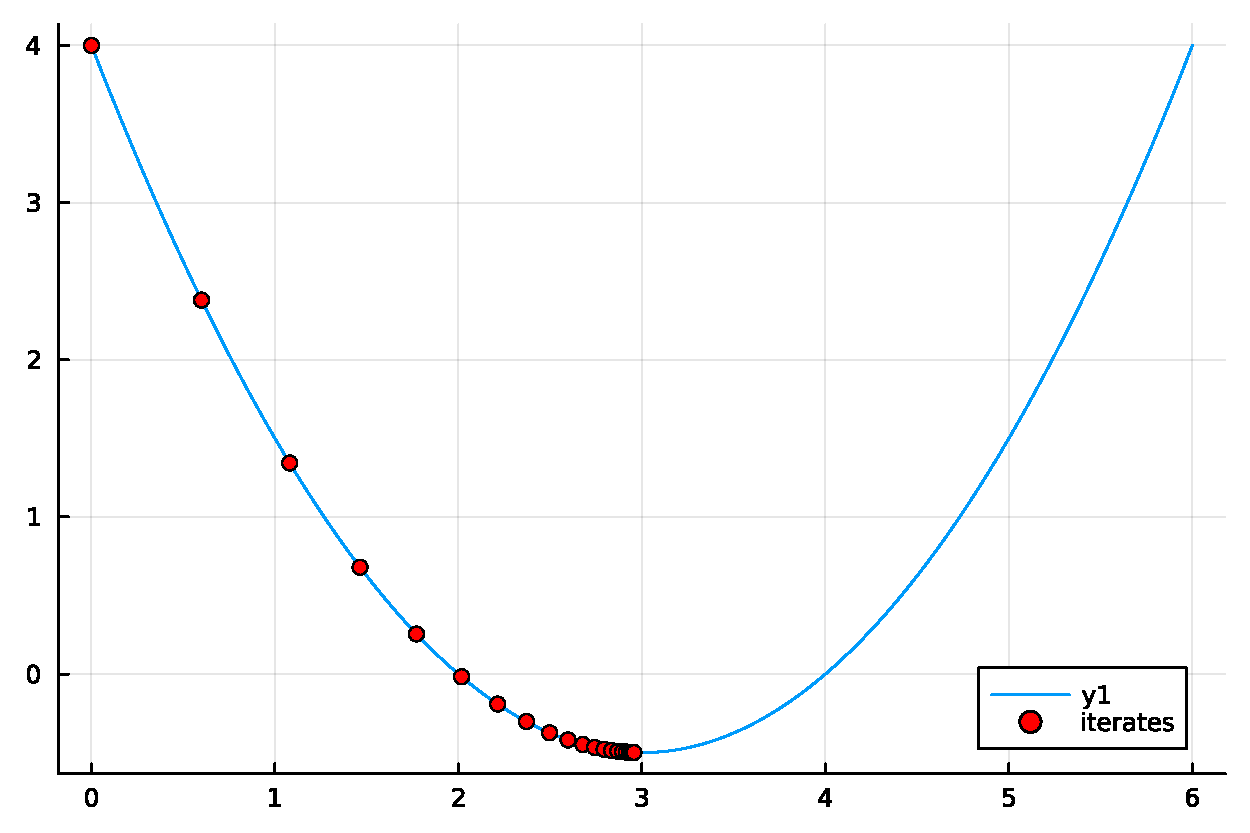
\includegraphics[width=.85 \linewidth]{crude1}
    \caption{$\alpha = 0.2$, iteration complexity = 20}
    \label{fig:crude1}
  \end{subfigure}%
  \begin{subfigure}{.5\textwidth}
    \centering
    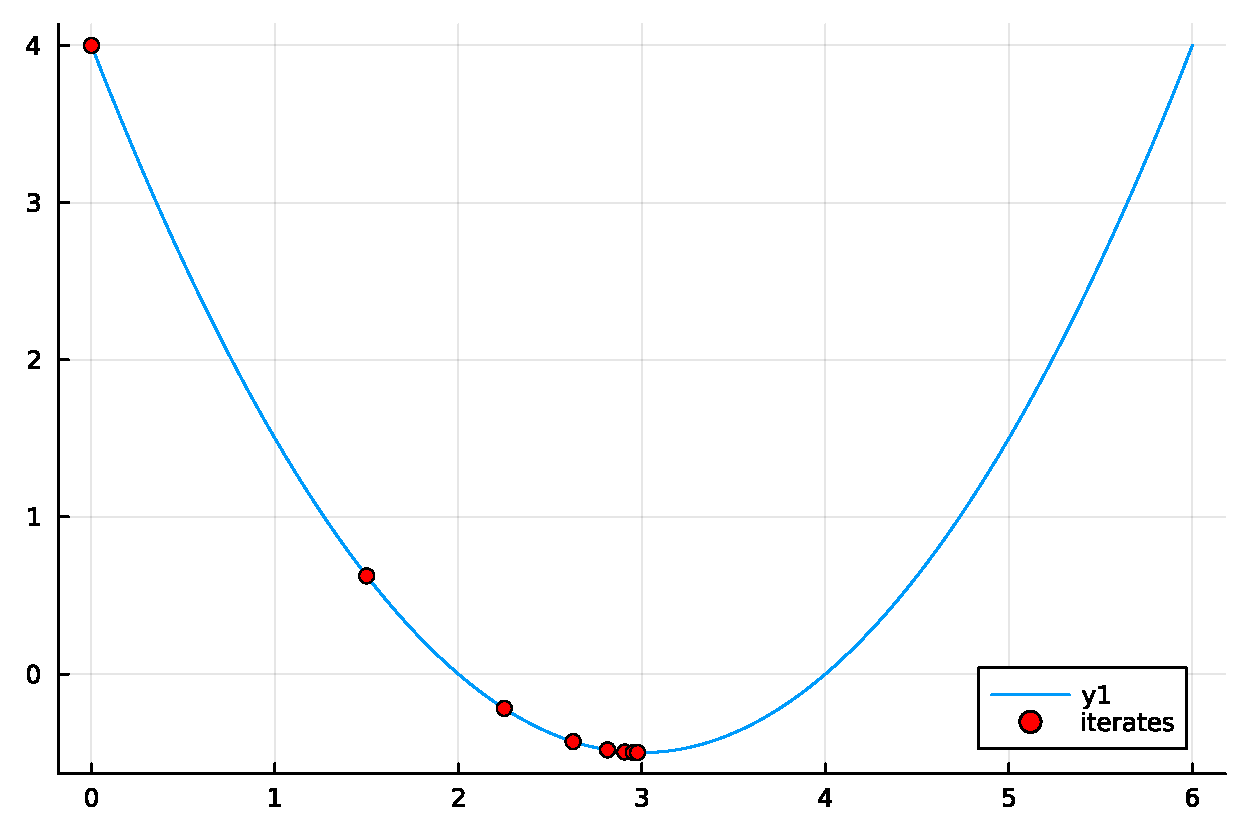
\includegraphics[width=.85 \linewidth]{crude2 }
    \caption{$\alpha = 0.5$, iteration complexity = 7}
    \label{fig:crude2}
  \end{subfigure}
  \begin{subfigure}{.5\textwidth}
    \centering
    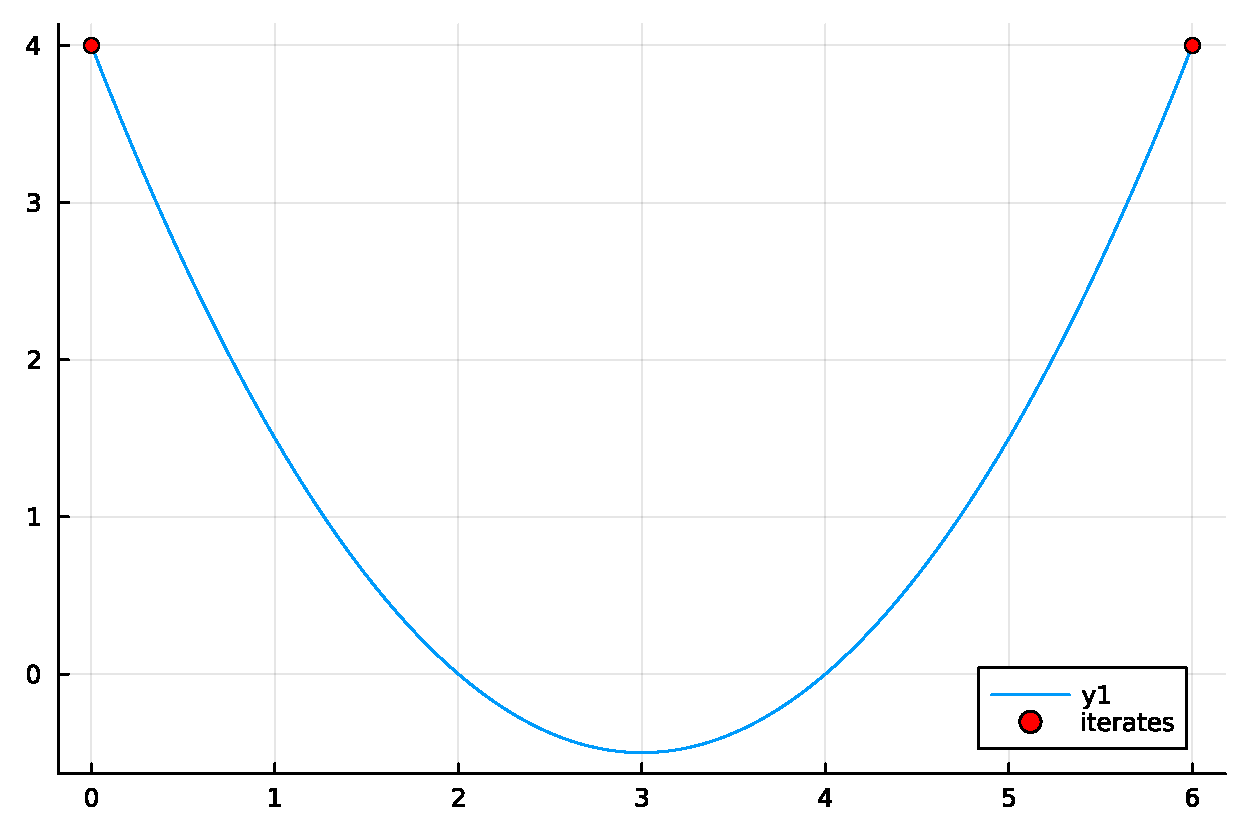
\includegraphics[width=.85 \linewidth]{crude3 }
    \caption{$\alpha = 2$, does not converge}
    \label{fig:crude3}
  \end{subfigure}
  \caption{Performance of 3 GD variants of different step sizes solving a quadratic function}
\label{fig:test}
\end{figure}

% \begin{figure}[htp]
%   \centering
%   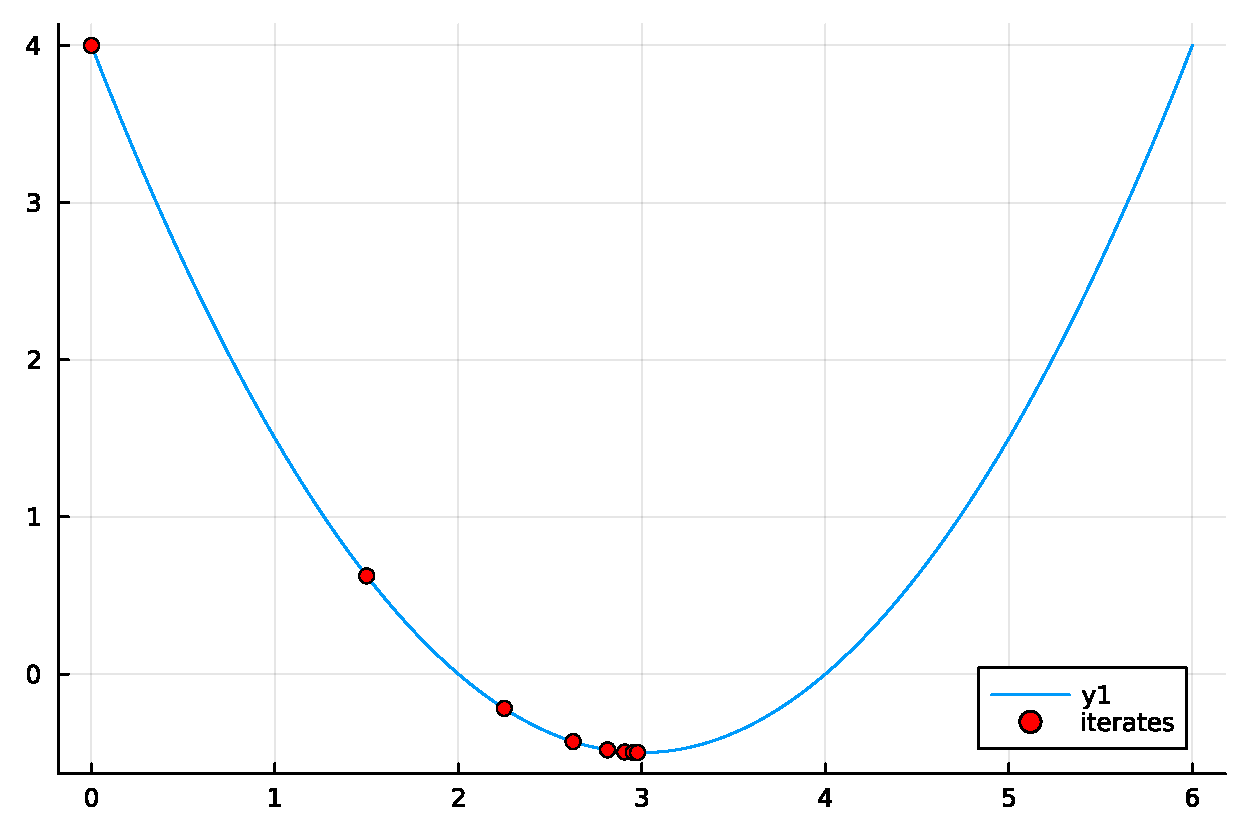
\includegraphics[width=.6\textwidth]{crude2}\hfill
%   \caption{$\alpha = 0.5$, iteration complexity = 21}
%   \label{fig:crude2}
% \end{figure}
% \begin{figure}[htp]
%   \centering
%   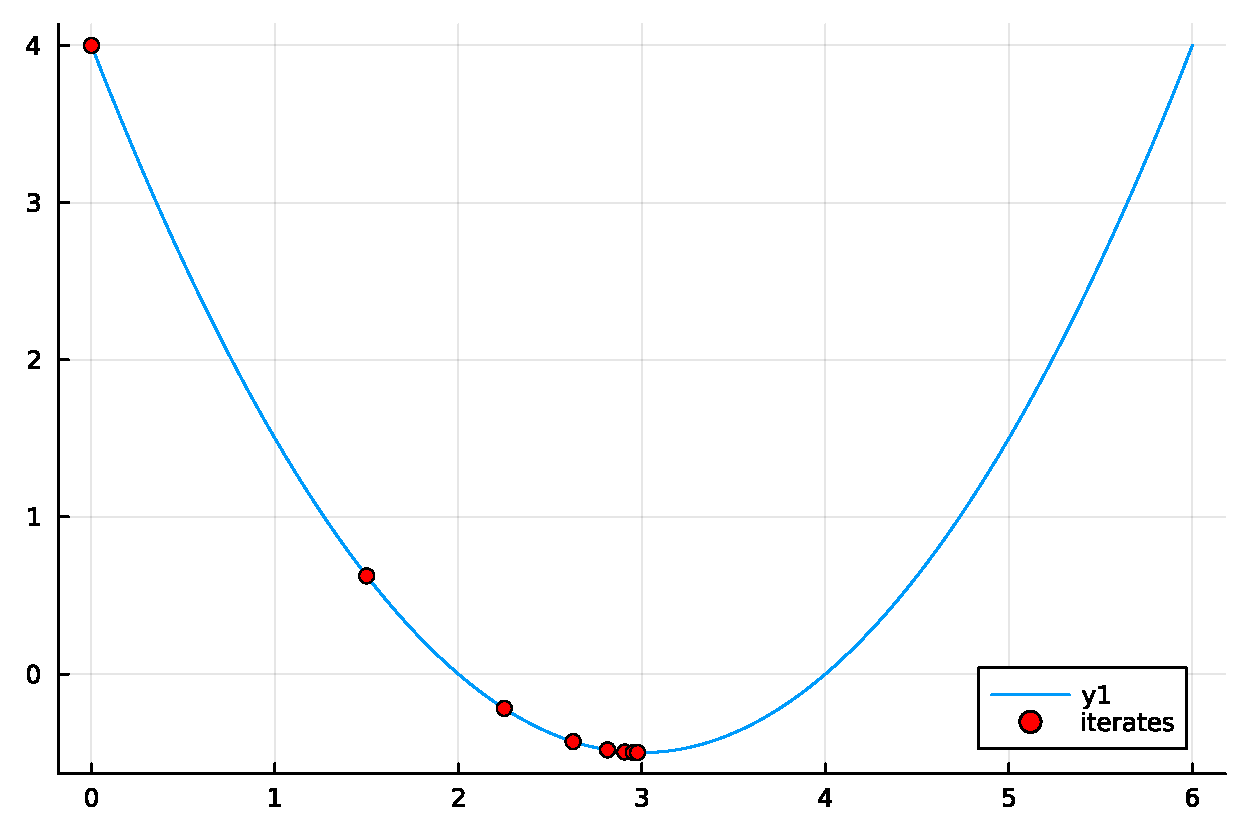
\includegraphics[width=.6\textwidth]{crude2}\hfill
%   \caption{$\alpha = 2$, does not converge}
%   \label{fig:crude3}
% \end{figure}

It can be seen how different tunings on the same algorithm can achieve drastically different speed optimizing a function, or whether it can solve for the minimum at all. Considering there exist many other first order methods in addition to the three in 1.1, each infinitely adjustable by changing the step size or by changing the number of past iterations used, being able to predict how an algorithm will perform can speed up the process of finding the best performing algorithm which can find a more accurate solution can be found and in fewer iterations. And while the example is of a simple function where overshoot can easily be identified and the number of iteration needed is small, the benefit of using an optimal algorithm only increases as the problem gets larger and more complex. In the application of training large language and self-driving models, the training process has taken place for many years and will continue as more training data is available and the models' continous improvement is desired. This training uses vast amounts of time and computational power, as a result, even a small improvement in the performance of the algorithm used can speed up the training process while reducing the energy needed.

Considering the quadratic function example, while it yielded an analysis of the algorithms' performance, it required solving the optimization problem. Not only would solving any problem large enough to warrant being optimized numerically in the first place computationally expensive, any benefit of finding a superior algorithm at solving a problem is negated as said problem has already been solved. Additionally, any analysis result is applicable only to one function and cannot be reliably used to derive a first-order method's performance on any other problem.

Due to these limitations, it is more efficient to analyze algorithms' performance at solving a broader set of problems. As a result of their widespread application, popular iterative gradient-based algorithms have been extensively analyzed. A frequently cited attempt is the Adam algorithm \cite{adam}, in which the performance of algorithms are compared using experiments and emperical evidence. There exists a different approach to quantifying the performance of algorithms, presented in \cite{drori2012}, \cite{taylor2016}, and \cite{lessard2016}, which aims to find a mathematically provable performance guarantee of an algorithm over a class of functions. This worst-case analysis is referred to as algorithm analysis: Given that a characteristic that a set of functions might share (such as being convex or quadratic), algorithm analysis would return the worst-case performance measure that guarantees the algorithm analyzed would perform as good or better at solving every function within said set.

\section{Julia programming language}

Algorithm Analysis is written in the Julia programming language, a high-level programming language designed specifically for high-performance numerical computing. Julia's compiler performance has been benchmarked to be faster than many other languages used for numerical computing while rivalling C, a language often used for its high efficiency \cite{julia}. Julia accomplishes this while being a high-level language with simple syntax rules that resembles existing popular languages, making it easy to develop and to understand.

Julia was also chosen as it is designed for numerical computing, supporting matrices as well as UTF-8 encoding, making it possible to use scientific notation: variables and functions as they exist in the code and as the user inputs them into the program can use math symbols or Greek letters. This makes Julia excel at communicating mathematical concepts, which simplifies both the process of coding the program and understanding its mathematical underpinnings.

Julia was also chosen as it is open-source and available for free. As Algorithm Analysis is a package designed for expert and novice users alike to install and use, it made sense to choose Julia as it is available on many of the popular platforms such as macOS, Windows, and Linux.

\section{Analysis Example}
To perform algorithm analysis with Algorithm Analysis, the user needs to follow the folliowing 3 steps:
\begin{enumerate}
	\item Choose from a supported list the class of function to be optimized.
	\item Define an algorithm to be analyzed .
	\item Specify a performance measure.
\end{enumerate}
In the Lyapunov-based method to analyzing algorithms and in Algorithm Analysis, a function class is defined as every functions which share a trait. In example \ref{ex_analysis}, the class of function is sector bounded between $m=1$ and $L=10$, which include any function $f$ that satisfy the condition:
\begin{equation}
  (\nabla f(x) - m(x-x_*))^\tp (\nabla f(x) - L(x-x_*)) \leq 0
\end{equation}
where $x_*$ is the global minimum of the function $f$
\begin{figure}[h!]
	\begin{lstlisting}[mathescape]
m,L = 1,10
$ \alpha $ = 2/(L+m)
@algorithm begin

	f = DifferentiableFunctional{R$ ^n $}()
	xs = first_order_stationary_point(f)
	f' $ \in $ SectorBounded(m, L, xs, f'(xs))

	x0 = R$ ^n $()
	x1 = x0 - $ \alpha $*f'(x0)

	x0 => x1

	performance = (x1-xs)^2
end

@show rate(performance)
\end{lstlisting}
\caption{Analysis Example}
\label{ex_analysis}
\end{figure} In the example code, the user:
\begin{itemize}
	\item Define the class of function \texttt{f} and its $\nabla f$, coded as \texttt(f') by calling one of the provided functions.
	\item Set the global minimum goal as a stationary point $ x_s $.
	\item Define an initial state $ x_0 $ and the algorithm with which its next state $ x_1$ is updated. In this example, the algorithm being analyzed is gradient descent with a step size $ \alpha = 2/11$.
	\item Set the performance measure as the norm distance between the initial state and the goal $ (x_0 - x_s)^2 $. The returned convergence rate guarantee is the rate at which the performance measure decreases after each iteration of the algorithm.
	\item Call the rate function to perform algorithm analysis.
\end{itemize}

With the calling of the rate function, Algorithm Analysis is ran automatically to return a rate of 0.6687164306640625. This is the converenge rate guarantee $\rho$ such that, for some performance measure $c>0$, it is upper bounded by $c \rho^k$ at each iteration $k$, for the provided algorithm and every function in the class. This guaranteed convergence rate using ``big-oh'' notation means that the performance measure converges with a minimum rate of $O(\rho^k)$. Throughout the process, the user never has to modify the package beyond providing its input or understand how Algorithm Analysis operate, making it an accessible tool.

\begin{figure}[hbtp]
  \begin{lstlisting}
  rate(performance) = 0.6687164306640625
  \end{lstlisting}
  \caption{Analysis result}
  \label{ex_result}
\end{figure}

\section{Overview} \label{sectionOverview}

% JuPE performs worst-case algorithm analysis when three main inputs are provided: the class of functions in question, the algorithm being analyzed, and a performance measure. The package then performs the algorithm analysis and returns the fastest guaranteed convergence rate.

% To use JuPE, an iterative first-order algorithm needs to be defined as an input to the program by specifying how it is updated. The class of function is provided by detailing the characteristic of the set, and a performance measure is defined. Throughout the process, the user never has to change the code of the package or understand how JuPE works, making it an easy to use black box tool.

%, such as 1 strong 10 smooth convex function, which can be how far the iterate \(x_k\) is from the goal \(x_*\) or any quadratic combinations of the iterates
Ater the introduction, in \Cref{chapter:literature}, the existing literature of approaches to analyzing algorithms and implementation into a program is presented. \Cref{chapter:lyapunov} discusses the Lyapunov-based mathematical method that Algorithm Analysis utilizes. In \Cref{chapter:code}, the main contribution of this thesis is presented: how a dommain-specific language is developed to support Algorithm Analysis's functionality. Finally in \Cref{chapter:result}, the analysis process and result are presented.

% \comment{Reference the specific chapters, such as Chapter~\ref{chapter:literature} (see the reference label at the beginning of that chapter for how to make the rerence).}
 \chapter{Literature Review}

In recent years, numerous studies have been conducted comparing the performance of optimization algorithms, particularly in machine learning and deep learning contexts. These comparisons often focus on convergence speed, accuracy, and robustness across various models and datasets. In \cite{adam}, Kingma and Ba presented the Adam (Adaptive Moment Estimation) algorithm. In order to prove its efficiency improvement above existing algorithms, the authors designed and conducted experiments where they are used to solve popular machine learning models and recorded the convergence rate of each. The result of these experiments provided emperical evidence that Adam performed better compared to its peers and gave a general idea of Adam's performance.

On the other hand, there exist in the literature approaches to performing algorithm analysis. In 2014, Drori and Teboulle first introduced the method of representing a class of function with constraints, reformulating the problem of analyzing an optimization method into a semidefinite program (SDP) whose size is proportionate with the number of iterations the algorithm is run.\cite{drori2012}. The paper coined the term Performance Estimation Problem (PEP) and showed that by solving a convex semidefinite problem (SDP), a worst-case numerical bound on an algorithm's performance solving that class of function can be derived. Taylor, Hendrickx and Glineur built upon this work by introducing the ideas of creating a finite representation for a class of smooth strongly convex functions using closed-form necessary and sufficient conditions. This work culminated in a way to perform algorithm analysis to derive the performance bound in the form of a guarantee that after a finxed number of iterates, how close the last iterate is to the goal.

In \cite{iqc}, Megretski and Rantzer demonstrated how integral quadratic constraints (IQCs) can be used to unify and simplify the analysis of system stability and performance. The paper shows how a complex system can be described using certain IQCs and presents a stability theorem for systems described by IQCs.

Computer programs have been developed to perform algorithm analysis using the PEP methods, which are PESTO \cite{pesto}, a MATLAB toolbox, and PEPit \cite{pepit}, a Python package. The program is able to perform algorithm analysis and generate a worst-case performance guarantee for algorithms and function classes from a supported list. PESTO and PEPit follows the PEP methodology and first presented an automatic way to analyze gradient-based algorithms.

JuPE implements the approach presented in \cite{tutorial}, which uses IQCs to represent the gradient of the algorithm and transforms the problem of deriving a performance guarantee to a convex SDP similar to the PEP approach. However, this approach instead uses Lyapunov functions to create a small and fixed size SDP, unlike that created by the PEP approach which grows in size for each iteration an algorithm is run, and proves that the performance measure inputted by the users decreases at a guaranteed rate throught out the optimizing process.

The main contribution of this thesis paper is to create a computer program named JuPE similar PESTO and PEPit that aims to provide an accessible and fast way to analyze the performance of first-order methods for a guaranteed convergence rate. By developing a domain-specific compiler inside the Julia programming language, JuPE simplifies the process of defining an optimization algorithm, provides a systemic way to represent abstract concepts such as algorithm iterate or the gradient of an abstract function, and make accessible the analysis of optimization algorithms. 
\chapter{Lyapunov-based approach}

JuPE performs algorithm analysis by using the technique layed out by Van Scoy and Lessard in \cite{tutorial}. While JuPE is a blackbox tool, understanding the mathematical approach on which it is based is prequisite to understanding the package's code and functionalities.

The technique is based on the idea that certifying whether a convergence rate of an algorithm optimizing a function can be guaranteed is itself an optimization problem. This approach, which will be discussed over the sections of this chapter, 1) represents the algorithm being analyzed in state-space, 2) replaces the nonlinear gradient with constraints derived from interpolation conditions of a function class, 3) form an optimization problem using Lyapunov functions and constraints and solve it to certify whether a certain convergence rate can be guaranteed.
% The steps of this technique, which will be discussed in detail over the sections of this chapter, consists of 
% 1) viewing the algorithm as a Lur'e problem, 2) Replacing the nonlinear gradient with interpolation conditions that represent the class of smooth strongly convex functions, 3) Use lifting matrices to tighten to the interpolation condition representations, and 4) Prove whether a convergence rate is guaranteed by solving a convex semidefinte program.
%%%%%%%%%%%%%%%%%%%%%%%%%%%%%%%%%%%%%%%%%%%%%%%%%%%%%%%%%%%%%%%%%%%%%%%%%%%%%%%%
\section{Iterative algorithms as Lur'e problems}

The first step in the technique is to view optimization algorithms from a control theory perspective: As iterative gradient-based algorithms uses the gradient of the function to update \(x\), they can be reformulated into a linear time-invariant (LTI) system (how the algorithm update) in feedback with a static nonlinearity (the gradient of \(f\)) at point \(x\). Using a block diagram, the algorithm can be seen as:

\begin{figure}[h]
    \centering
	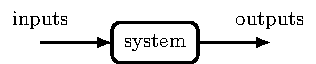
\includegraphics[width = .3 \textwidth]{block-diagram}
    \caption{Block diagram representation of iterative algorithms}
    \label{plot_result}
\end{figure}

Here, \(G\) represents the LTI system, while \(y\) and \(u\) are input and output of the gradient nonlinearity. For example, (FG) equation \ref{eqn:FG} can be rewritten to match this view as:
\begin{subequations} \label{eqn:FG2}
	\begin{align}
	  x_{k+1}     &=x_k-\alpha u_k \label{eq_FGstate},       \\
	  y_{k+1} &=x_{k+1}+\beta (x_{k+1}-x_k), \label{eq_FGinterpolated point}, \\
	  u_k &= \nabla f(y_k) \label{eq_FGggradient}
	\end{align}
	\end{subequations}
The algorithm can then be put into state-space representation with augmented state $\xi _k = (x_k, x_{k-1})$ as:
\begin{subequations} \label{eqn:FGss }
	\begin{align}
	  \xi_{k+1} &= \bmat{(1+\beta) & -\beta\\ 1 & 0}\xi_k  + \bmat{-\alpha\\ 0}u_k \label{eq_FGssstate}, \\
	  y_k &= \bmat{1+\beta & \beta}\xi_k, \label{eq_FGssinterpolation},\\
	  u_k &= \nabla f(y_k) \label{eq_FGssgradient}
	\end{align}
	\end{subequations}

It should be noted that the function $f$ is n-multivariate, and iterate $x_k$ is n-dimensional $\in \Re^n$, represented by a 1xn vector. $\xi $ therefore is a 2xn matrix.

The LTI system \(G\) can be expressed with four matrices that change in value depending on the algorithm and size depending on the number of past states used to update \(x\). For (GD), (FG), and (HB) as they are described in 1.1, these matrices are:

Beyond the three listed examples, this step can be applied to any other first order methods. Deriving an LTI system represented by matrices out of an algorithm not only creates a representation easy to understand and operate on, but also in next sections enable the representation of the past states of an algorithm and the forming of a Lyapunov function.

\section{Interpolation condition}

% For the remainder of this paper, we will focus on the only class of function currently supported by JuPE, m strong L smooth convex function \(f \in \) \(F_{m,L}\).
\subsection*{Function class interpolation conditions}

In the field of robust control theory utilized by this Lyapunov-based approach, while an LTI system is relatively simple, the nonlinearity representing the gradient of the function cannot be efficiently solved. As a result, the Lyapunov-based approach replaces the nonlinearity with a characterization of the class of function. Since the algorithm is being analyzed at discrete iterates, the characterization of a function class can be done using interpolation conditions, a set of conditions on the linearity's input and output $y$ and $u$. The interpolation conditions of a function class provide necessary and sufficient conditions under which there exists a function in that class that interpolates a given finite set of iterate-gradient pairs. These interpolation conditions depends on the characteristics of and can be derived from the function class. The interpolation condition of m strong L smooth convex functions was first formulated in \cite{taylor2016} and reformatted in \cite{tutorial} as:

\begin{theorem}[\cite{taylor2016}, Thm. 4; \cite{tutorial}, Thm. 3]
	\label{thm:interpolation_condition}
	Given index set \(I\), a set of triplets \({(y_k, u_k, f_k)}_{k \in I}\) is \(F_{m,L}-interpolable\), meaning there exists a function \(f \in F_{m,L}\) satisfying \(f(y_k) = f_k\) and \(\nabla f(y_k) = u_k\) if and only if:

	\(2(L-m)(f_i - f_j) - mL||y_i - y_j||^2 + 2(y_i - y_j)^{T}(mu_i - Lu_j) - ||u_i - u_j||^2 \geq 0\) for \(i ,j \in I\)

\end{theorem}

As an example, if we define $x_0$ as the initial iterate of an algorithm optimization a 1 strong 10 smooth convex function (\(f \in \) \(F_{1,10}\)), $\nabla f(x_0)$ as the gradient of $x_0$ at $f$, $x_s$ as the minimizer where  $\nabla f(x_s) = 0$, we can define set $I$ of \ref{thm:interpolation_condition} as including $s$ and $0$ and get the inequality:
\begin{equation} \label{eqn:int_cond}
	-20||x_0||^2 -20||x_s||^2 + 40\innerproduct{x_0}{x_s} + 22\innerproduct{\nabla f(x_0)}{x_0} - 22\innerproduct{\nabla f(x_0)}{x_s} - 2||\nabla f(x_0)||^2 \geq 0
\end{equation}
when satisfied interpolates 1 strong 10 smooth convex functions. Theorem \ref{thm:interpolation_condition} can be rewritten as:
\begin{equation} \label{eqn:int_cond2}
	% \begin{align}
	%   tr \bmat{y_i \\ y_j \\ u_i \\ u_j}^TH\bmat{y_i \\ y_j \\ u_i \\ u_j} + h^T\bmat{f_i \\ f_j} \geq 0 \\
	%   tr \bmat{y_i \\ y_j \\ u_i \\ u_j}^T\Lambda H\bmat{y_i \\ y_j \\ u_i \\ u_j} + \Lambda h^T\bmat{f_i \\ f_j} \geq 0 \\
	%   tr \Lambda \bmat{y_i \\ y_j \\ u_i \\ u_j}\bmat{y_i \\ y_j \\ u_i \\ u_j}^TH + \Lambda h^T\bmat{f_i \\ f_j} \geq 0
	\Lambda\bmat{-mL & 2mL & -mL & 2(m+L) & -2(m+L) & -2m}\bmat{||y_i||^2 \\ \innerproduct{y_i}{y_j} \\ ||y_j||^2 \\ \innerproduct{\nabla f(y_i)}{y_j} \\ \innerproduct{\nabla f(y_j)}{y_i} \\ ||\nabla f(y_j)||^2} \geq 0
	% \end{align}
\end{equation}
% With $H = \bmat{-mL & mL & m & -L\\mL & -mL & -m & L\\m & -m & -1 & 1\\-L & L & 1 & -1}$ 

For all $\Lambda \in \Re^{4x4}$ such that $\Lambda_{i,j} \geq 0$. We perform this transformation in order to represent the gradient of smooth strongly convex functions or any function class with interpolation condition inside the optimization problem: For a function \(f \in F_{m,L}\) satisfying \(f(y_k) = f_k\) and \(\nabla f(y_k) = u_k\), if $\Lambda $ is constrained so that every of its element is non-negative, then the left hand side of the inequalities defined by \ref{eqn:int_cond2} is non-negative. Following this transformation, \ref{eqn:int_cond} can be transformed into:
\begin{equation}
	\Lambda\bmat{-2 & 4 & -2 & 2.2 & -2.2 & -0.2}\bmat{||x_k||^2 \\ \innerproduct{x_k}{x_s} \\ ||x_s||^2 \\ \innerproduct{\nabla f(x_k)}{x_k} \\ \innerproduct{\nabla f(x_k)}{x_s} \\ ||\nabla f(x_k)||^2} \geq 0
\end{equation}
The constraints on $\Lambda $ are added to the optimization problem, and the resulting nonnegative inequalities \ref{eqn:int_cond2} are combined and used in the formulation of Lyapunov functions discussed in the next section.
% Whether an algorithm being analyzed uses the gradient of multiple past states to update, or the state-space representation of an algorithm include the gradient of more than one iterate, there might exists multiple iterate-gradient pairs, each creating an inequality for their interpolation. By combining these inequalities, each scaled by a nonnegative optimization variable $\lambda $, a tight representation of the function class can be created. The inequalities in \ref{eqn:int_cond} can be combined to create:

% Basing on this theorem, [\cite{tutorial}, Cor 4] presented a non-negative linear combination of inequalities to create a tight representation of the class of function, which can be rewritten in a way easier to implement into code as:

% \begin{corollary}[\cite{tutorial}, Cor. 4]
% 	Given a function \(f \in F_{m,L}\) and let \(y_k,...,y_{k-l}\) be a sequence of iterates; \(u_{k-i} = \nabla f(y_{k-i})\) and \(f_{k-i} = f(y_{k-i})\) for \(i \in 0,...l\). Then the inequality:
	
% 	holds for all \(\Lambda \in \mathbb{R}^{(l+2) * (l+2)}\) and \(\Lambda >= 0\), and \(\Pi(\Lambda)\) and  \(\pi(\Lambda)\) are defined as:

% \end{corollary}

% The left hand side of each constraint, such as \ref{eqn:int_cond}, is scaled by an optimization variable $\Lambda$ and added to the Lyapunov functions. The optimization varibles $\Lambda$s are constrained in the optimization problem to be greater or equal to zero if the left hand side is a vector or scalar or postive semidefinite if the left hand side is a matrix

\subsection*{Transpose interpolation condition}

\section{Lyapunov function certification}

\cite{tutorial} presents the Lyapunov based approach, in which a Lyapunov function is created using the state-space representation of the algorithm, an optimization variable $P$, and the constraints created by the interpolation conditions. A convergence rate guarantee is found by solving for $P$ so that the Lyapunov function would satisfy 2 linear matrix inequalities. The mathematical basis of JuPE follows this approach with some modification. 

Define $\mathbf{x_k} = \xi _k - \xi _s $, the Lyapunov function would take the form of:
% = \bmat{x_{k} - x_s \\ x_{k-1} - x_s}$, the Lyapunov function would take the form of:

\begin{equation}
	V(\mathbf{x}) = tr(\mathbf{x_k}^TP\mathbf{x_k}) \label{eqn:Lyapunov}
\end{equation}

Where $P$ is a 2x2 optimization variable. If given an algorithm with state-space representation $\xi _k$ and whose Lyapunov function satisfy the conditions:
\begin{subequations} \label{eqn:Ly_ineq}
	\begin{align}
	  ||\xi _k - \xi _s||^2 - V(\mathbf{x_k}) \leq 0,      \\
	  V(\mathbf{x_{k+1}}) - \rho ^2V(\mathbf{x_k}) \leq 0
	\end{align}
\end{subequations}

Then the convergence rate of that algorithm is guaranteed to be larger than $\rho $ for every function in the function class. While the Lyapunov function is quadratic in $\mathbf{x_k}$, due to the characteristics of matrix trace, we can see that $V(\mathbf{x})$ is linear in $\mathbf{x}^T\mathbf{x}$, reducing the inequalities to linear matrix inequalities. For gradient descent where the augmented state $\xi_k$ is just the state $x_k$, the Lyapunov function can be simplified into:
\begin{subequations}  \label{eqn:Vx}
	\begin{align}
		V(\mathbf{x_{k}}) = tr[(x_k - x_s)^TP(x_k - x_s)]\\
						  = tr[P(x_k - x_s)(x_k - x_s)^T]\\
						  = tr[P(x_kx_k^T - x_sx_k^T - x_kx_s^T + x_sx_s^T)] \\
						  = \bmat{P & -2P & P}\bmat{||x_k||^2 \\ \innerproduct{x_k}{x_s} \\ ||x_s||^2}
	\end{align}
\end{subequations}
Where $x_kx_s^T = x_sx_k^T = \innerproduct{x_k}{x_s}$. Similarly, $V(\mathbf{x_{k+1}})$ can be defined as:
\begin{subequations}  \label{eqn:Vx+}
	\begin{align}
		V(\mathbf{x_{k+1}}) = V(x_k - \alpha \nabla f(x_k)) \\
						  	= tr[(x_k - \alpha \nabla f(x_k) - x_s)^TP(x_k - \alpha \nabla f(x_k) - x_s]\\
						  	= tr[P(x_k - \alpha \nabla f(x_k) - x_s)(x_k - \alpha \nabla f(x_k) - x_s)^T]\\
						  	= \bmat{P & -2P & P & 2P\alpha & -2P\alpha & P\alpha^2}\bmat{||x_k||^2 \\ \innerproduct{x_k}{x_s} \\ ||x_s||^2 \\ \innerproduct{\nabla f(x_k)}{x_k} \\ \innerproduct{\nabla f(x_k)}{x_s} \\ ||\nabla f(x_k)||^2}
	\end{align}
\end{subequations}

The Lyapunov functions inequalities can now be completed by adding the constraints created by the interpolation conditions. For each constraint created by the interpolation conditions, an optimization variable $\Lambda $ is created and constrained to be nonnegative element-wise if it is a vector or scalar, positive semidefiinite if it is a matrix. The left hand side of \ref{eqn:int_cond2} can be added to each Lyapunov function. Continuing the example, substituting the updated state $x_k$ for the initial state $x_0$ in the left hand side of the constraint, the final Lyapunov functions for gradient descent would be:

\begin{subequations} \label{eqn:Ly_ineq}
	\begin{align}
		L1 = \bmat{1-P-2\Lambda \\ -2+2P+4\Lambda \\ 1-P-2\Lambda \\ 2.2\Lambda \\ -2.2\Lambda \\ -0.2\Lambda}^T\bmat{||x_k||^2 \\ \innerproduct{x_k}{x_s} \\ ||x_s||^2 \\ \innerproduct{\nabla f(x_k)}{x_k} \\ \innerproduct{\nabla f(x_k)}{x_s} \\ ||\nabla f(x_k)||^2} \leq 0 \\
		\bmat{P-P\rho^2-2\Lambda \\ -2P+2P\rho^2+4\Lambda \\ P-P\rho^2-2\Lambda \\ 2P\alpha+2.2\Lambda \\ -2P\alpha-2.2\Lambda \\ P\alpha^2-0.2\Lambda}^T\bmat{||x_k||^2 \\ \innerproduct{x_k}{x_s} \\ ||x_s||^2 \\ \innerproduct{\nabla f(x_k)}{x_k} \\ \innerproduct{\nabla f(x_k)}{x_s} \\ ||\nabla f(x_k)||^2} \leq 0
	\end{align}
\end{subequations}

By using Lyapunov functions, we have reduced the optimization problem to a pair of linear matrix inequalities in the variables $P$ and $\Lambda$ which are added to our optimization problem. The optimization problem can now be solved for any $\rho$ whether there exist values for optimization varibles $P$ and $\Lambda $ so that the inequality constraints added to the problems are satisfied, proving whether a convergence rate guarantee of $\rho$ is feasible. The smallest convergence rate guarantee can be found by performing bisection search on $\rho$ between 0 and 1 and checking if the optimization problem is feasible at each search step.

% By expanding \ref{eqn:xTPx}, we can see that $\mathbf{x}^T\mathbf{x}$ is a linear function of real variable, which can be transformed into a linear form. For example, for a gradient descent algorithm with step size $\alpha $ and $\xi _{k+1} - \xi _s = \bmat{x_k - \alpha * \nabla f(x_k) - x_s \\ x_k - x_s}$, we can define $o = \bmat{||x_k||^2 \\ <x_k, x_s> \\ ||x_s|| \\ ||\nabla f(x_k)||^2 \\ <\nabla f(x_k), x_k> \\ <\nabla f(x_k), x_s>}$ and $\mathbf{X}$ and $\mathbf{X^+}$as:
% \begin{subequations}  \label{eqn:X}
% 	\begin{gather}
% 		\mathbf{X}^T*o	= (\xi _k - \xi _s)^T*P*(\xi _k - \xi _s) \\
% 		\mathbf{X} = \bmat{1 & 0 & 0 & 0 & 0 & 0 \\ 0 & 1 & 0 & 0 & 0 & 0 \\ 0 & 0 & 1 & 0 & 0 & 0 \\ 0 & 0 & 0 & 0 & 0 & 0 \\ 0 & 0 & 0 & 0 & 0 & 0 \\ 0 & 0 & 0 & 0 & 0 & 0} \\
% 		\mathbf{X^+} = \bmat{1 & 0 & 0 & 0 & 0 & 0 \\ 0 & 1 & 0 & 0 & 0 & 0 \\ 0 & 0 & 1 & 0 & 0 & 0 \\ 0 & 0 & 0 & -\alpha ^2 & 0 & 0 \\ 0 & 0 & 0 & 0 & -2\alpha & 0 \\ 0 & 0 & 0 & 0 & 0 & -2\alpha}
% 	\end{gather}
% \end{subequations}

% Through this transformation, the updated state can be expressed is a linear function of $\mathbf{X}$ for any algorithm $\mathbf{X^+} = A\mathbf{X}$ where A is a real matrix. Similarly, $||\xi _k - \xi _s||^2$ can also be transformed into linear form $\mathcal{P} $ so that $\mathcal{P}^T*o = ||\xi _k - \xi _s||^2$. \ref{eqn:Ly_ineq} can now be transformed into:
% \begin{subequations} \label{eqn:newLy_ineq}
% 	\begin{align}
% 	  \mathcal{P} - tr(\mathbf{X}^TP) \leq 0      \\
% 	  tr(\mathbf{X}(A^TPA- \rho ^2P)) \leq 0
% 	\end{align}
% \end{subequations}






% \begin{equation} \label{eqn:Lyapunov}
% 	V(x) = <P, X[x; u]> = <X^T P, [x; u]>
% \end{equation}


\chapter{Code Structure}

To in order to perform algorithm analysis with JuPE, the user need to follow the folliowing 3 steps:
\begin{enumerate}
	\item Specify the class of function to be optimized.
	\item Choose an algorithm to be analyzed from a supported list or entering a new one 
	\item Specify a performance measure
  \end{enumerate}
JuPE then perform analysis automatically and return a worst-case guarantee convergence rate.

This chapter goes into the core component code that enables JuPE and the analysis process.

%%%%%%%%%%%%%%%%%%%%%%%%%%%%%%%%%%%%%%%%%%%%%%%%%%%%%%%%%%%%%%%%%%%%%%%%%%%%%%%%
\section{Core Components}

In a broad sense, JuPE's analysis functionality is a set of instructions that use the input to create and solve an optimization problem to derive a performance certification. This optimization problem consists of the Lur'e representations of the algorithms as well as the interpolation conditions. This requires the program to be able to keep track of and differentiate between variables representing concepts such as functions, gradients or values amongst others. Not only are these variables then able to be used to create optimization problems, it should also be simple for the user to define them as they provide input for the program. JuPE uses data structures to intuitively represent these concepts.

\subsection*{Expressions}
Expressions are data structures acing as the small building block upon which every other concepts are built. Expressions must belong to one of the defined types, which are: . Algebra can be done on expressions, and each expression contains information on its decomposition of expressions. 

\subsection*{Oracles}
As JuPE perform analysis over sets of functions using only constraints on the \(\nabla (f)\) block of \ref{}, the block can be treated as a blackbox. These blackboxes are represented by oracles, data strucutres containing the relation and constraint information between expressions. Each oracle represent a class of function and can only exist if there exist interpolation conditions for said class.

Oracles can be sampled at an expression to return another expression, establishing the relation information between the two expressions and create every constraints on them following the function class' interpolation conditions.

\subsection*{States}
States are linear combinations of expressions representing the states of an algorithms. By inputing how the states are updated, the "next" and "prev" fields of the expressions inside the states are stored.

\subsection*{Constraints}

\section{Analysis Process}

Using this inequality, constraint matrices \(M\) and \(m\) can be constructed:
When the interpolation conditions are satisfied, \(M\) and \(m\) are positive definite, meaning they are symmetric and and its eigenvalues are positive.



%%%%%%%%%%%%%%%%%%%%%%%%%%%%%%%%%%%%%%%%%%%%%%%%%%%%%%%%%%%%%%%%%%%%%%%%%%%%%%%
%% APPENDICES
%%%%%%%%%%%%%%%%%%%%%%%%%%%%%%%%%%%%%%%%%%%%%%%%%%%%%%%%%%%%%%%%%%%%%%%%%%%%%%%
\appendices
% \chapter{Background}

Use appendices to provide background information that the reader may already know, but is useful in case they need a refresher. A thesis on control, for example, may have an appendix on the linear--quadratic regulator, or some linear algebra.

\backmatter


%%%%%%%%%%%%%%%%%%%%%%%%%%%%%%%%%%%%%%%%%%%%%%%%%%%%%%%%%%%%%%%%%%%%%%%%%%%%%%%
%% BIBLIOGRAPHY
%%%%%%%%%%%%%%%%%%%%%%%%%%%%%%%%%%%%%%%%%%%%%%%%%%%%%%%%%%%%%%%%%%%%%%%%%%%%%%%
\addcontentsline{toc}{chapter}{References}
\renewcommand\bibname{References}
\bibliography{references}

\end{document}